% !TeX root = ../tesis.tex

\section{Microcito}
\label{section:Res_Microcito}
Make a short summary of the content of the thesis and then your conclusions. Also explain your future steps on this project 

%
%
%
\begin{figure}[h!]
	\centering
	\sidesubfloat[Second image]{\hspace{-0.3cm}{
			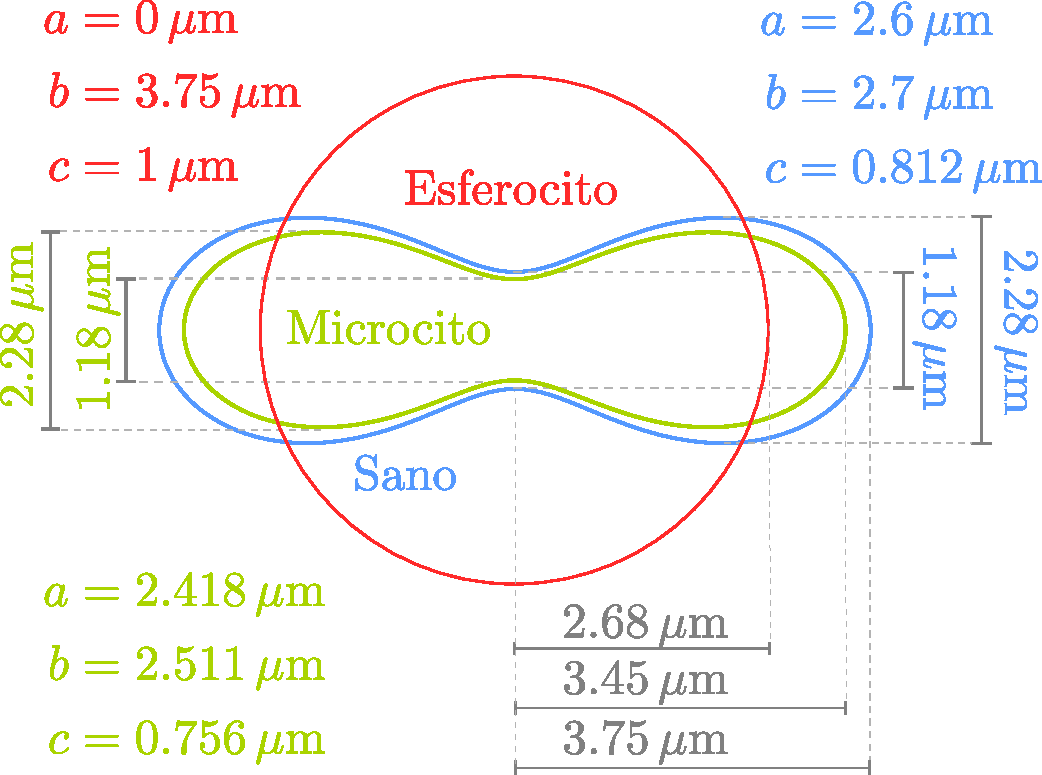
\includegraphics[width=0.48\textwidth]{../../Figuras/4-Resultados/Eritrocito_sano_esferocito_microcito_corte.pdf}\label{}}}\hspace{0.1cm}
	\sidesubfloat[First image]{\hspace{-0.5cm}{	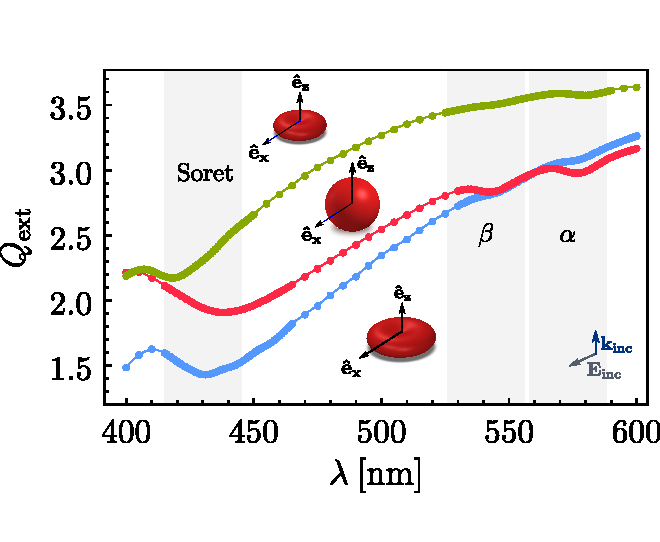
\includegraphics[width=0.45\textwidth]{../../Figuras/4-Resultados/Qext_Micro.pdf}\label{}}}
	\vspace{-0.1cm}
	\caption{}
	\label{}
\end{figure}
%

%
\begin{figure}[h!]
	\centering
	\sidesubfloat[First image]{\hspace{-0.5cm}{	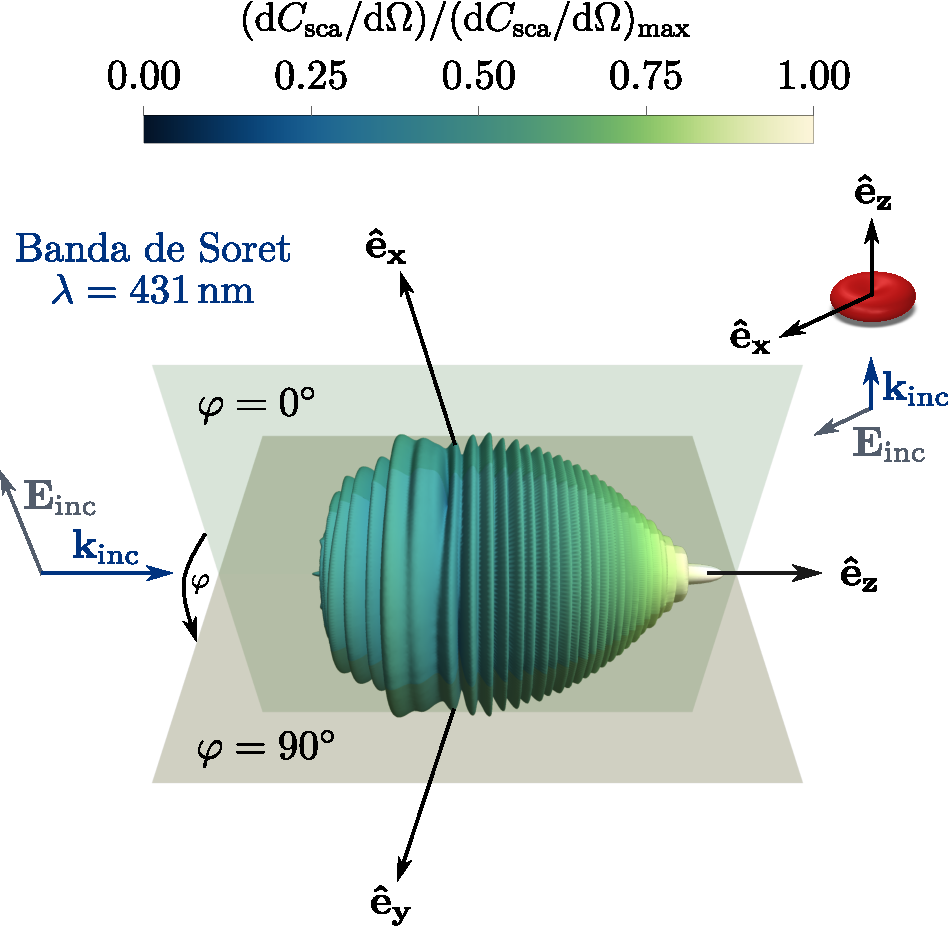
\includegraphics[width=7.3cm]{../../Figuras/4-Resultados/FFdistribution431_Micro.pdf}\label{}}}\hspace{0.1cm}
	\sidesubfloat[Second image]{\hspace{-0.5cm}{
			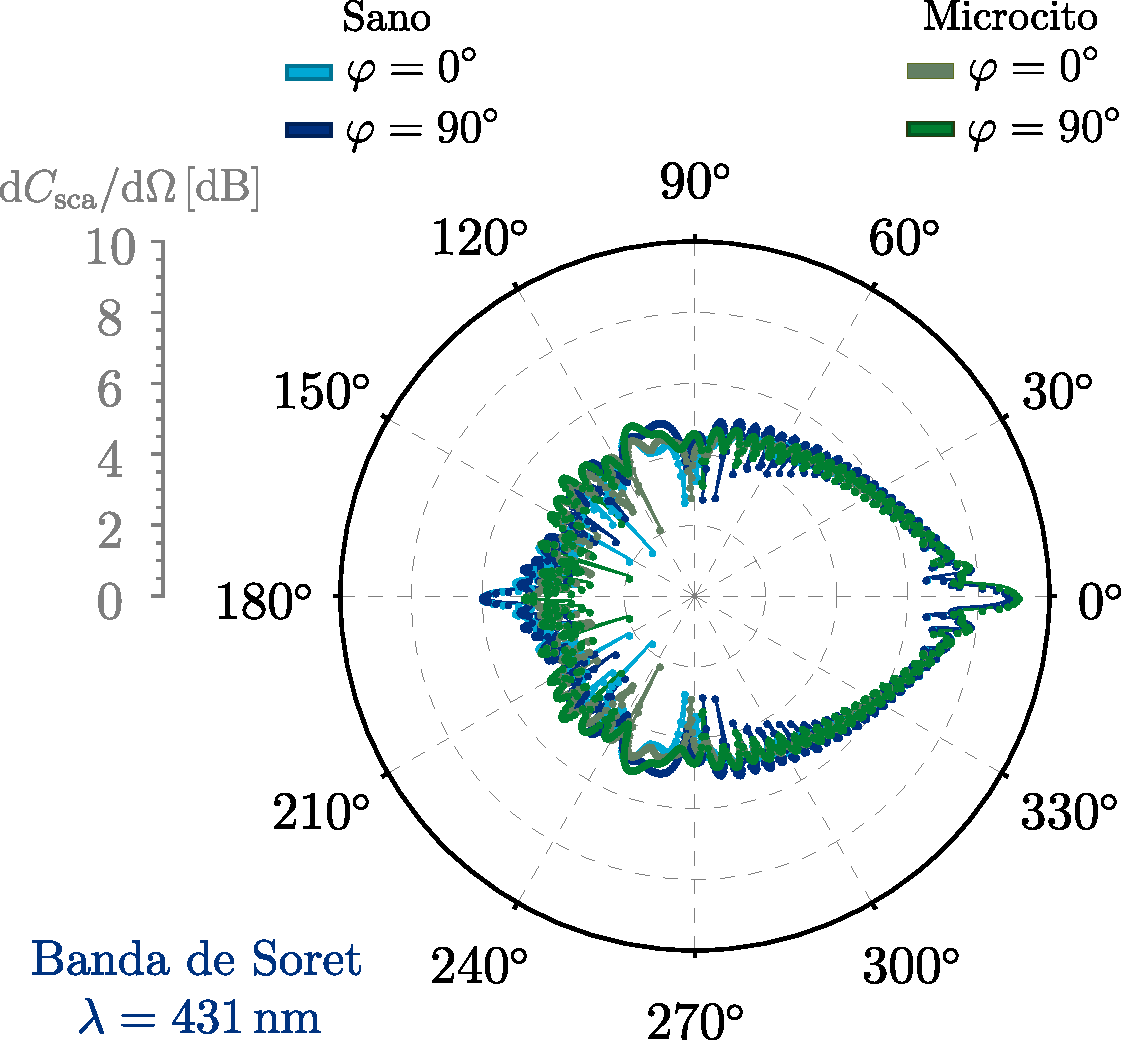
\includegraphics[width=8cm]{../../Figuras/4-Resultados/polarplot431FFComEsfMicro.pdf}\label{}}}\vspace{-0.1cm}
	\\
	\vspace{0.7cm}
	
	\sidesubfloat[Third image]{\hspace{0.3cm}{
			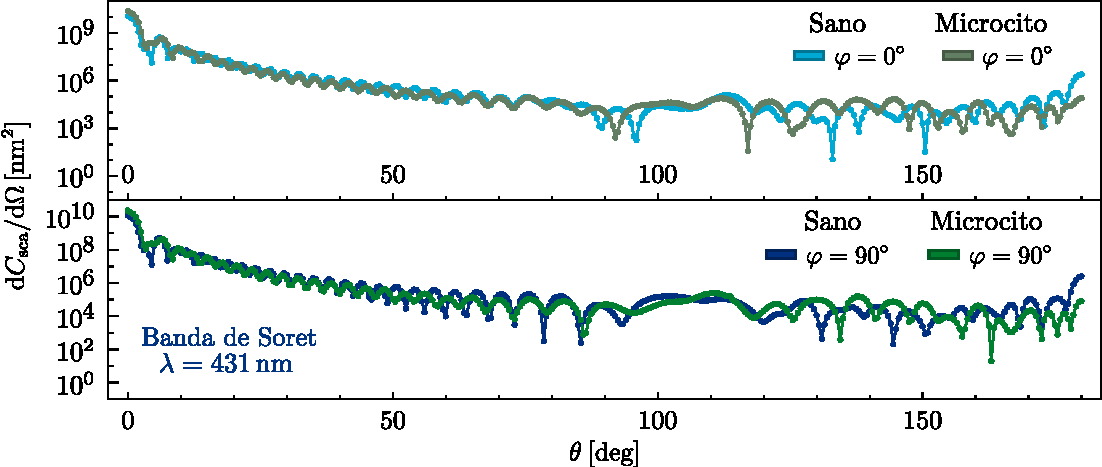
\includegraphics[width=14cm]{../../Figuras/4-Resultados/linearplot431FFMicro.pdf}\label{}}}\vspace{-0.1cm}
	\caption{\textbf{a)} }
	\label{}
\end{figure}
%